\chapter{Experimentació} 
\label{cap:exp}
La principal tasca d'aquest projecte fou la de dissenyar els experiments de manera que els resultats foren el més significatius possible i que l'única diferència que hi hagués entre el reconeixement emprant els dos mètodes fou la de la segmentació del cos central del text en les imatges. D'aquesta manera es pot conèixer exactament quines són les diferències quantitatives entre els dos mètodes, calculant la diferència en l'error de reconeixement obtingut a l'emprar les dues alternatives.\\

A banda de la publicació original on s'explicava l'apro\-xi\-ma\-ció que utilitza aprenentatge supervisat per a la segmentació del text \cite{DBLP:conf/pris/Gorbe-MoyaEZB08}, els mateixos autors publicaren a la revista \emph{IEEE Transactions on Pattern Analysis and Machine Intelligence} (PAMI), el 2011, una comparativa entre dos estratègies per a la modelització dels models morfològics. Una basada únicament en HMM i l'altra un híbrid entre HMM i ANN \cite{espana2011improving}. L'interessant d'aquesta publicació per a l'objectiu d'aquest projecte és que utilitzava la segmentació del cos central supervisada (secció \ref{sec:seg_nn}) en ambdós casos i donava més detalls sobre l'entrenament complet del reconeixedor (model de llenguatge, models morfològics, etc) que no pas l'article original on s'explica la segmentació del cos central utilitzant aprenentatge supervisat.\\

El disseny dels experiments ací descrits busca reproduir els resultats publicats en \cite{espana2011improving} del reconeixedor basat únicament en HMM utilitzant la segmentació del cos supervisada i comparar-los en un altre reconeixedor basat també en HMM i utilitzant la segmentació heurística. Malauradament, molts dels detalls de l'entrenament que dugué als resultats publicats eren desconeguts, així com els detalls d'implementació exactes de les ferramentes utilitzades.\\

Per solucionar aquests contratemps i intentar reproduir de la manera més exacta possible els resultats, els autors de la publicació ens proveïren de les característiques extretes a partir de les línies del corpus IAMDB, així com del model de llenguatge, construït a partir dels corpus de Brown, LOB i Wellington.

\section{Mesura d'avaluació}
Per a quantificar el comportament dels dos sistemes comparats en la tasca de reconeixement en el corpus d'IAMDB s'utilitza el \emph{Word Error Rate} (WER). Aquesta mesura d'error compara els errors en les paraules en la transcripció del sistema amb la transcripció de referència.
\begin{equation}\label{eq:wer}
\text{WER} =  \frac{\text{Insercions} + \text{Substitucions} + \text{Esborrats}}{\text{Nombre de paraules en la referència}} \cdot 100
\end{equation}

Un WER igual a zero sols s'aconsegueix si la transcripció produida pel sistema és igual a la transcripció de referència. En la fòrmula \ref{eq:wer}, ``Insercions'', ``Substitucions'' i ``Esborrats'' fa referència al nombre mínim de paraules que han de sofrir una d'aquests transformacions en la transcripció obtinguda pel sistema per tal d'obtenir la transcripció de referència. Aquesta mesura d'error és molt semblant al \emph{Character Error Rate} (CER), on les operacions es compten a nivell de símbol en lloc de a nivell de paraula. Cal observar que és possible obtenir un WER major al $100\%$ si la transcripció té més errors que paraules hi han en la transcripció de referència. Això és degut a que el sistema pot produir una transcripció amb més paraules que el text de referència.

\section{Preprocessament de les imatges}
En els dos reconeixedors entrenats, s'aplicà el següent preprocessament a les línies de text d'IAMDB.
\begin{enumerate}
\item Neteja de la imatge. L'objectiu d'aquesta etapa és la de netejar el soroll en les imatges utilitzades. En el cas de la segmentació basada en aprenentatge supervisat, prèviament s'eliminava el soroll utilitzant una xarxa neuronal multicapa que donat una graella de la imatge centrada en un píxel, obtenia el valor del píxel central restaurat. Aquesta xarxa neuronal s'entrenava a partir d'imatges amb soroll i la seva imatge equivalent sense soroll. Més detalls sobre aquest mètode poden trobar-se en \cite{DBLP:conf/pris/Gorbe-MoyaEZB08,espana2011improving}. En el cas de la segmentació heurística, el mètode utilitzat per a la neteja de la imatge és l'explicat en \cite{Pastor07}. En primer lloc, la imatge en blanc i negre es normalitza a l'escala $[0,255]$, siguent 0 el píxel més obscur de la imatge original i 255 el més clar. D'aquesta manera s'augmenta el contrast a la imatge original. Després s'aplica un filtre mediana, amb el qual el valor de cada píxel és determina com la mediana dels valors d'una finestra centrada en aquest píxel.

\item Correcció del \emph{slope}. L'objectiu és corregir l'angle que forma la línia de text amb la línia horizontal de la imatge (veure figura \ref{fig:slope_correction}). En el cas del reconeixedor que feia ús de la segmentació heurística, la correcció es fa seguint la tècnica descrita en \cite{Pastor07}. Aquesta tècnica consisteix en girar la imatge provant diferents angles de rotació, trobar la seva projecció horizontal i escollir aquell angle que produisca una columna amb el valor acumulat dels píxels major. En el cas del reconeixedor que feia ús de la segmentació basada en aprenentatge automàtic, la tècnica ve descrita en l'article \cite{DBLP:conf/pris/Gorbe-MoyaEZB08}. Aquesta tècnica consisteix en trobar la línia de referència inferior, amb un mètode semblant al descrit en \ref{sec:seg_nn}, calcular l'angle entre aquesta línia i la base de la imatge i corregir aquest angle rotant la imatge.

\item Correcció del \emph{slant}. L'objectiu d'aquesta etapa és la de corregir l'angle que forma cada lletra amb la línia vertical de la imatge (veure figura \ref{fig:slant_correction}). En ambdós casos la tècnica utilitzada és la descrita en \cite{pastor2004projection,Romero05,Pastor07}. Aquesta tècnica consisteix en transformar la imatge aplicant una transformació \emph{shear} aplicant diferents angles, calcular la projecció vertical de la imatge i escollir aquell angle amb el qual s'obté una major desviació típica en la projecció.

\item Segmentació del cos central. En un dels reconeixedors entrenats s'utilitza la segmentació heurística descrita a la secció \ref{sec:seg_heur} i en el segon la segmentació supervisada descrita a la secció \ref{sec:seg_nn}.

\item Normalització de l'altura d'ascendents i descendents. Aquesta etapa té com a objectiu normalitzar l'altura dels símbols independentment del seu autor, context, situació, etc. En ambós reconeixedors, la tècnica és la mateixa. Una vegada segmentat el cos central, per a cada columna de píxels, la zona d'ascendents s'escala a un $20\%$ de la imatge i la de descendents a un $10\%$.

\item Extracció de característiques. En ambdós reconeixedors, s'utilitza la tècnica descrita en \cite{toselli2004integrated,Pastor07}. Es recorre la imatge utilitzant una finestra lliscant amb 20 graelles i s'extreu per a cada graella el nivell mitjà de gris normalitzat, la derivada horizontal del nivell de gris i la derivada vertical del nivell de gris. De manera que de cada finestra d'anàlisi s'obtenen 60 característiques.
\end{enumerate}
Tot i que les etapes de netja de la imatge i correcció del \emph{slope} també varien, proves preliminars dutes a terme pels autors que desenvoluparen els mètodes basats en xarxes neuronals, mostren que les diferències entre els mètodes utilitzats en aquests casos no són significatives. D'aquesta manera, l'única variable amb un efecte significatiu sobre el resultat del reconeixement que es veu alterada és la segmentació del cos central.

\begin{figure}
\centering
\begin{subfigure}[b]{0.8\textwidth}
\centering
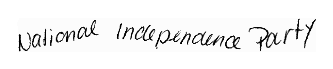
\includegraphics[width=\textwidth]{images/slope_orig.eps}
\caption{}\label{fig:slope_correction_orig}
\end{subfigure}\\
\begin{subfigure}[b]{0.8\textwidth}
\centering
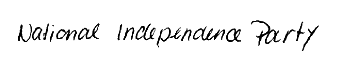
\includegraphics[width=\textwidth]{images/slope_corr.eps}
\caption{}\label{fig:slope_correction_result}
\end{subfigure}
\caption{Exemple de la correcció del \emph{slope} \cite{Pastor07}.}\label{fig:slope_correction}
\end{figure}

\begin{figure}
\centering
\begin{subfigure}[b]{0.8\textwidth}
\centering
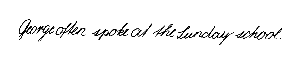
\includegraphics[width=\textwidth]{images/slant_orig.eps}
\caption{}\label{fig:slant_correction_orig}
\end{subfigure}\\
\begin{subfigure}[b]{0.8\textwidth}
\centering
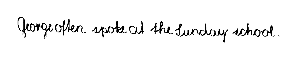
\includegraphics[width=\textwidth]{images/slant_corr.eps}
\caption{}\label{fig:slant_correction_result}
\end{subfigure}
\caption{Exemple de la correcció del \emph{slant} \cite{Pastor07}.}\label{fig:slant_correction}
\end{figure}

\section{Model del llenguatge}
El model del llenguatge utilitzat en ambdós sistemes fou un proveït per els autors de l'article on es descriu el mètode de segmentació basat en xarxes neuronals i que és semblant al que ells utilitzaren en la publicació \cite{espana2011improving}. De nou, l'idea d'utilitzar un model del llenguatge el més semblant possible era poder reproduir els resultats obtinguts en la publicació.\\

El model del llenguatge està basat en $n$-grames, un modelatge molt popular en la literatura a l'hora de construir models de llenguatge \cite{ManningSchuetze99}. En aquest cas, el model de llenguatge estava format per bigrames entrenats a partir de textos de tres corpus distints: el corpus Brown (secció \ref{sec:corpus_brown}); el corpus LOB, excloent aquells textos que contenien línies incloses en el conjunt de test del corpus IAMDB  (secció \ref{sec:corpus_lob}) i el corpus Wellington (secció \ref{sec:corpus_wellington}). La ferramenta utilitzada per a la generació del model del llenguatge fou la popular SRI Language Modeling Toolkit \cite{stolcke2002srilm}, utilitzant el suavitzat de Kneser-Ney modificat \cite{chen1999empirical}.\\

S'utilitzaren $51560$ frases del corpus LOB, $51763$ del corpus Brown i $20592$ del Wellington. Per tal de modelar el fet que el text en les imatges de IAMDB està fragmentat en línies, les frases anteriors foren fragmentades aleatòriament per tal de simular les línies i s'obtingueren $400000$ d'aquests fragments. Finalment, s'afegiren també les $6161$ línies del conjunt d'entrenament del corpus IAMDB.\\

De totes les línies anteriors, sols s'utilitzaren les $20000$ paraules més comunes per tal de construir el model del llenguatge i fer un sistema amb un diccionari obert, de manera que es simula un entorn sense restriccions en el vocabulari. Un altre factor important d'aquest model del llenguatge és el fet que totes les lletres foren convertides a minúscules.

\section{Models morfològics}
L'habitual combinació de Models Ocults de Markov i Models de Mixtures Gaussianes fou emprada per tal de modelar el model morfològic de cada símbol. En els dos sistemes comparats, s'utilitzà la ferramenta Hidden Markov Model Toolkit (HTK) \cite{young1993htk} per construir aquests models. Les distribucions de Gauss en cada mixtura tenien una matriu de covariances diagonal i els Models Ocults de Markov tenien una topologia esquerra-dreta estricta (veure figura \ref{fig:hmm_left_right}). En total s'entrenaren 78 models morfològics, un per cada símbol ocorregut en les dades d'entrenament d'IAMDB.\\

Els models morfològics utilitzats en el cas de la segmentació utilitzant xarxes neuronals foren els mateixos que els utilitzats en la publicació anterior, proveïts per els seus autors. De nou, l'objectiu era que els resultats obtinguts foren el més semblants possibles als publicats. Aquest eren models de 8 estats i una mixtura de 64 gaussianes en cada estat. Aquesta configuració fou estimada a partir de provar diferents combinacions de paràmetres i escollint aquella amb un millor comportament en el corpus de validació.\\

\begin{figure}
\centering
\includegraphics[width=0.8\textwidth]{images/hmm_left_right.ps}
\caption{Topologia esquerra-dreta estricta d'un Model de Markov.}\label{fig:hmm_left_right}
\end{figure}

Pel que fa al sistema que utilitzava la segmentació heurística, també es provaren diferents combinacions del nombre de gaussianes en els GMM i el nombre d'estats en els HMM. La taula \ref{tab:estimacio_parametres_HMM} mostra els resultats d'aquesta estimació en un subconjunt de les línies de validació. En els dos sistemes, el paràmetre \emph{Grammar Scale Factor} (GSF) es fixà a 40 i el \emph{Word Insertion Penalty} (WIP) es fixà a 0. En \cite{espana2011improving} es comprova que amb un valor GSF d'entre 40 i 50 s'obtenien els millors resultats en el reconeixement, amb diferències no significatives estadísticament entre ells. Per a l'execució d'aquest experiment en el qual es buscava el nombre òptim d'estats en el HMM i del nombre de components en la Mixtura de Gaussianes, es van extreure 300 línies escollides aleatòriament de les 920 del conjunt de validació i es va escollir un llindar de poda \emph{beam} igual a 500 per a que el temps de reconeixement no fóra massa elevat.\\

\begin{table}
\centering
\begin{tabular}{cc|c|c|c|}
\cline{3-5}
& & \multicolumn{3}{c|}{Components de la mixtura}\\
\cline{3-5}
& & 16 & 32 & 64 \\ 
\cline{1-5}
\multicolumn{1}{|c|}{\multirow{3}{*}{Nombre d'estats}} & 7 & 54.91 & 46.75 & 42.84\\
\cline{2-5}
\multicolumn{1}{|c|}{} & 8 & 54.24 & 46.08 & \textbf{42.21}\\
\cline{2-5}
\multicolumn{1}{|c|}{} & 9 & 54.41 & 47.73 & 44.53\\
\cline{1-5}
\end{tabular}
\caption{WER en un subconjunt de validació utilitzant diferents paràmetres dels HMM en el sistema amb segmentació heurística. \emph{Beam} igual a 500.}\label{tab:estimacio_parametres_HMM}
\end{table}

S'observa en la taula \ref{tab:estimacio_parametres_HMM} que  la millor configuració de les provades fou aquella amb 8 estats per cada HMM i un total de 64 components gaussianes en els GMM. Aquesta fou la configuració utilitzada per conduir els experiments finals.

\section{Postprocessament al reconeixement}\label{sec:exper_filtre}
Una vegada reconegut el text se li aplica un filtre que intenta normalitzar les transcripcions. Aquest filtre va ser també utilitzat en la publicació \cite{espana2011improving} i fou proveït pels autors de la mateixa per tal d'obtenir uns resultats el més similar possibles amb els originals de la publicació.\\

Aquest filtre realitza les següents operacions sobre la transcripció.
\begin{itemize}
\item Els signes dobles de cita (\emph{``}, \emph{''}) i les barres verticals (\emph{|}) són substituides per signes simples de cita (\emph{`}, \emph{'}).
\item Les contraccions de l'anglès (p. ex: \emph{'s}, \emph{'d}, \emph{'nt}, etc.) són precedides amb un espai en blanc.
\item Els signes de puntuació (punts, comes, dos punts, punts i coma, etc.) són precedits amb un espai en blanc.
\item Els signes de cita i els parèntesis són seguits d'un espai en blanc.
\item Els espais en blanc seguits són substituits per un únic espai en blanc.
\end{itemize}

\section{Resultats finals}
La taula \ref{tab:comp_prhlt_elirf} mostra el WER obtingut amb les dues alternatives estudiades en aquest projecte i la seva diferència. Per a aquestes proves els paràmetres escollits foren els detallats anteriorment i amb un llindar de poda \emph{beam} igual a 800, el mateix que el que utilitzaren els autors de la publicació on es detalla \mbox{l'aproximació} basada en aprenentatge supervisat. Les columnes etiquetades com a ``No Filtre'' corresponen a les mesures d'error obtingudes abans d'aplicar el filtre descrit a la secció \ref{sec:exper_filtre}, les columnes etiquetades com a ``Filtre'' corresponen a les mesures d'error obtingudes una vegada el filtre s'havia aplicat a les transcripcions.\\

\begin{table}
\begin{center}
\begin{tabular}{ll|c|c|c|c|}
\cline{3-6} & & \multicolumn{2}{c|}{Validació} & \multicolumn{2}{c|}{Test}\\
\cline{3-6} & & No Filtre & Filtre & No Filtre & Filtre\\
\cline{1-6} \multicolumn{1}{|l}{} & Heurística & 40.93 & 38.74 & 46.85 & 45.54\\ 
\cline{1-6} \multicolumn{1}{|l}{} & Apr. Supervisat & \textbf{35.18} & \textbf{32.99} & \textbf{41.15} & \textbf{40.08}\\ 
\cline{1-6} \multicolumn{1}{|l}{} & Diferència & -5.75 & -5.75 & -5.70 & -5.46 \\ 
\hline 
\end{tabular} 
\caption{WER de les dues alternatives comparades. \emph{Beam} igual a 800.}\label{tab:comp_prhlt_elirf}
\end{center}
\end{table}

Pot observar-se que la diferència en tots els casos està al voltant de $-5.67$, sent aquesta per al conjunt de \emph{test} de $-5.46$ punts WER. Aquesta és la diferència entre el WER obtingut amb el sistema que utilitzava una segmentació basada en aprenentatge supervisat i el sistema basat en una aproximació heurística. Al ser aquesta diferència negativa en tots els casos, indica que el sistema utilitzant l'enfocament d'aprenentatge supervisat millora sempre a l'enfocament heurístic, per als experiments duts a terme sobre el corpus IAMDB. Aquest decrement de $-5.46$ punts absoluts en el WER, significa una millora (decrement) relativa del $11.99\%$ respecte al WER del sistema heurístic.